\documentclass{article}
\usepackage{graphicx}
\usepackage{subfigure}
\usepackage{dsfont}
\usepackage{amsthm}
\usepackage{amsmath}
\usepackage{cancel}
\usepackage[pdftex]{hyperref} 
\usepackage[]{mcode}
\usepackage{pdfsync}
\usepackage{fullpage}
\usepackage{color}

\pagestyle{plain}

\newcommand{\sgn}{\text{sgn}}
\newcommand{\abs}[1]{\left\vert#1\right\vert}
\newcommand{\mfile}[1]{{\bf \lstinputlisting{#1}}}
\newcommand{\bsol}{\begin{proof}[Solution]}
\newcommand{\esol}{\end{proof}}
\newcommand{\bq}{\begin{equation}}
\newcommand{\eq}{\end{equation}}
\newcommand{\R}{\mathbb{R}}
\newcommand{\N}{\mathbb{N}}
\newcommand{\E}{\mathbb{E}}
\newcommand{\e}{\epsilon}
\newcommand{\A}{\mathcal{A}}
\newcommand{\sY}{\mathcal{Y}}
\newcommand{\sX}{\mathcal{X}}
\newcommand{\PP}{\mathbb{P}}
\newcommand{\bO}{\mathcal{O}}
\newcommand{\blue}[1]{{\color{blue}{#1}}}

\newcommand{\softwarename}{MatIB}

\newtheorem{remark}{Remark}

\graphicspath{{./Figures/}}

\title{User Guide}
\author{Jeffrey Wiens, Brittany Froese, Dr. John Stockie}
\date{September 2011}

\begin{document}

\maketitle

\section{Introduction}\label{sec:intro}

\softwarename~ is a Matlab implementation of the immersed boundary (IB) method which is released under the MIT Open Source 
License \footnote{http://www.opensource.org/licenses/mit-license.php}\footnote{The MIT Open Source License only pertains to \softwarename 's codebase and not the algorithms used by \softwarename. Therefore, the original copyrights of these algorithms need to be respected when using \softwarename.}. The IB method was originally developed by Charles Peskin \cite{PeskinHearts} and has proven
to be a versatile method when simulating the interaction of a moving deformable membrane with a incompressible fluid. In \softwarename, we have implemented 
 Peskin's two-step numerical algorithm \cite{PeskinIB}. Although there are more sophisticated implementations of the IB method,
\softwarename~ is designed to reduce the barrier needed for researchers and students to study IB problems using the familiar Matlab environment.

We begin by establishing the mathematical equations that arise in the two-dimensional IB method for a closed membrane on the periodic domain 
$\Omega = [0,1]\times[0,1]$ which is parameterized using the Eulerian grid $\vec{x} = (x,y)$.  
The closed surface of the membrane at time $t$ is defined by the parametric curve
\[ \vec{\chi}(s,t) = (\chi_x(s,t),\chi_y(s,t)) \]
using the Lagrangian grid $s \in [0,1]$.

The fluid flow is governed by the incompressible Navier-Stokes equations:
\bq\label{eq:NSE}
\rho\left(\frac{\partial\vec{u}}{\partial t} + \vec{u}\cdot\nabla\vec{u}\right) = \mu \Delta \vec{u} - \nabla p + \vec{F},
\eq
\bq\label{eq:incompressible}
\nabla \cdot \vec{u} = 0
\eq
where $\vec{u}(\vec{x},t)=(u(\vec{x},t),v(\vec{x},t))$ is the fluid velocity, $\rho$ is the fluid density, $\mu$ is the dynamic viscosity, 
$p(\vec{x},t)$ is the pressure, and $\vec{F}(\vec{x},t)$ is the force. If the only force acting on the fluid comes from the immersed boundary, 
then $\vec{F}(\vec{x},t)$ is defined as 
\bq\label{eq:force}
\vec{F}(\vec{x},t) = \int\limits_\Gamma \vec{f}(s,t) \delta(\vec{x} - \vec{\chi}(s,t))\,ds
\eq
where
\begin{itemize}
\item $\vec{f}(s,t)$ is the force density on the membrane at the location $\vec{\chi}(s,t)$ and time $t$,
\item $\delta(\vec{x})$ is the 2D Dirac-delta function.
\end{itemize}
If we assume that the membrane is linked by linear springs, we can express the force density as
\bq\label{eq:forceDensity}
\vec{f}(s,t) = \sigma \frac{\partial}{\partial s}\left[\frac{\partial\vec{\chi}(s,t)}{\partial s}\left(1 - \frac{L}{\abs{\frac{\partial \vec{\chi}(s,t)}{\partial s}}}\right)\right]
\eq
where $\sigma$ is the spring constant and $L$ is the resting length of the membrane.
Lastly, the equation that governs the motion of the membrane is defined by 
\bq\label{eq:membrane}
\frac{\partial\vec{\chi}(s,t)}{\partial t} = \vec{u}(\vec{\chi}(s,t)) = \int\limits_\Omega \vec{u}(\vec{x},t)\delta(\vec{x}-\vec{\chi}(s,t))\,dx.
\eq

\section{How to use \softwarename}\label{sec:HowTo}

\subsection{Example: Elliptical Membrane}\label{sec:EllipticalMembrane}

In the folder \emph{examples/} in \softwarename's root directory, there contains a couple of example Matlab scripts demonstrating the use of \softwarename.
For example, the script \emph{examples/Elliptical Membrane/EllipticalMembrane.m}, plots a movie of how an elliptical membrane deforms in an initially 
stationary fluid. The membrane will oscillate and eventually settle into a circular state; see Figure~\ref{fig:ellipseProfile}.

\begin{figure}[htdp]
	\centering
	\subfigure[]{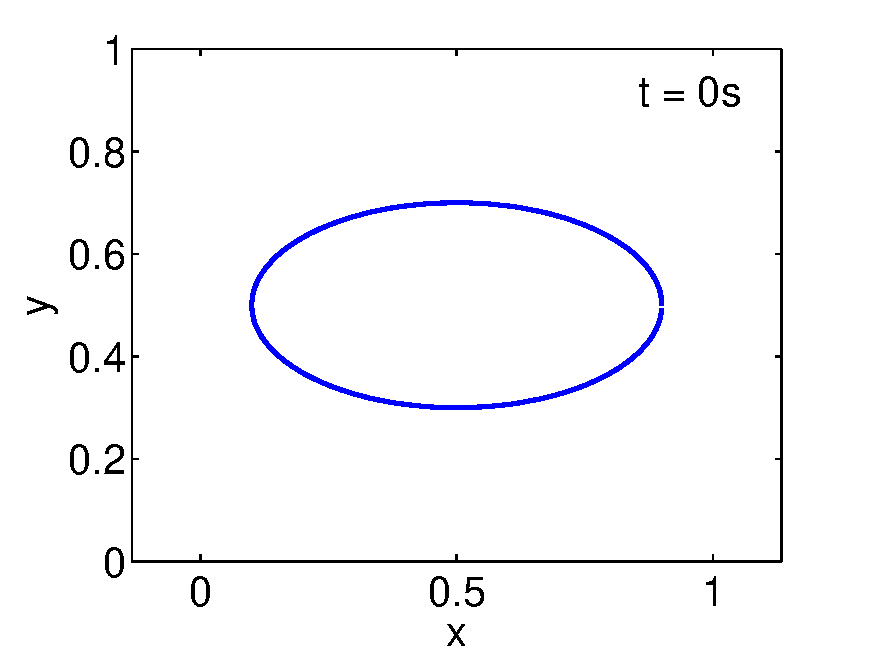
\includegraphics[width=.3\textwidth]{ellipse0000}\label{fig:ellipse0}}
	\subfigure[]{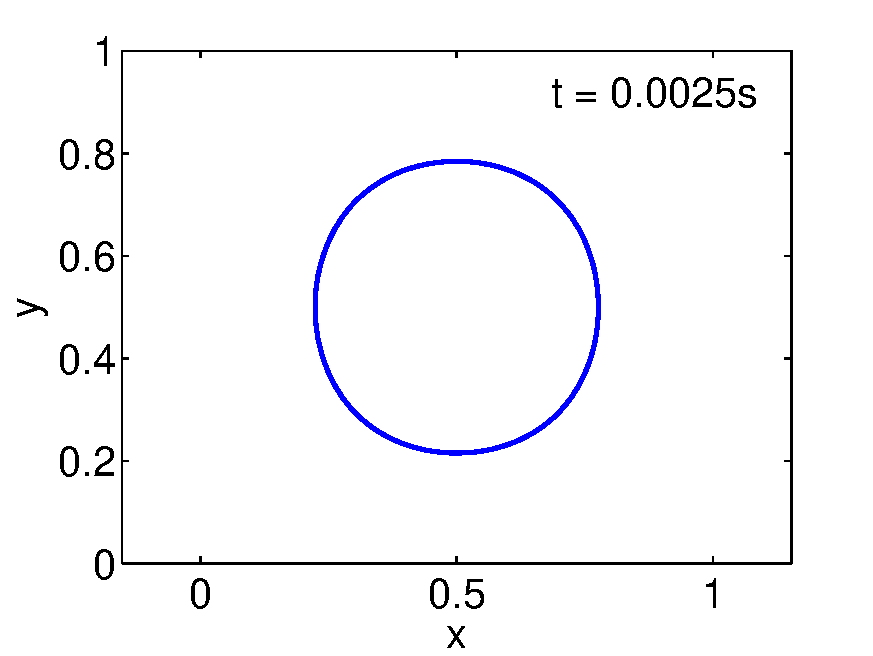
\includegraphics[width=.3\textwidth]{ellipse0025}\label{fig:ellipse1}}
	\subfigure[]{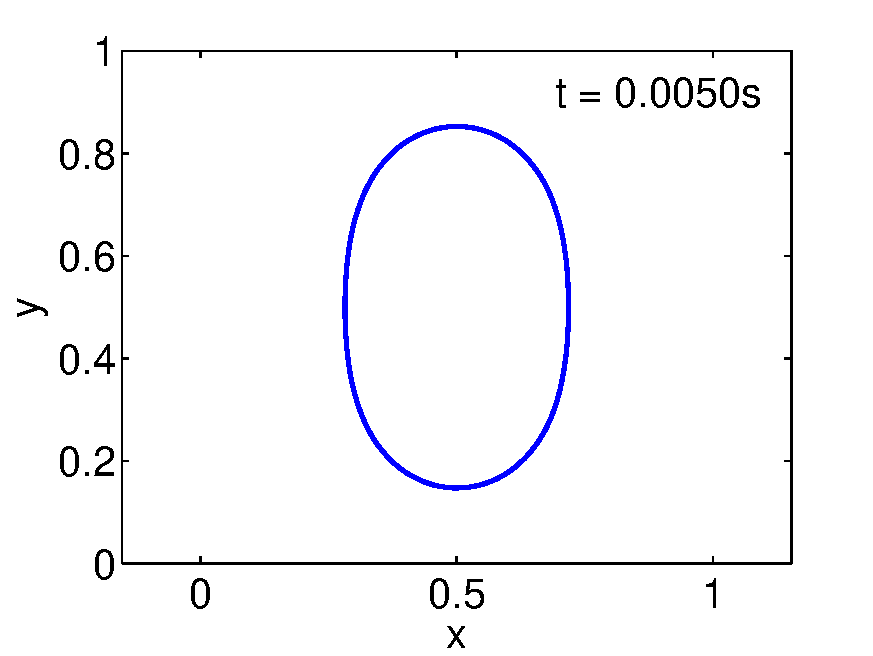
\includegraphics[width=.3\textwidth]{ellipse0050}\label{fig:ellipse2}}
  \subfigure[]{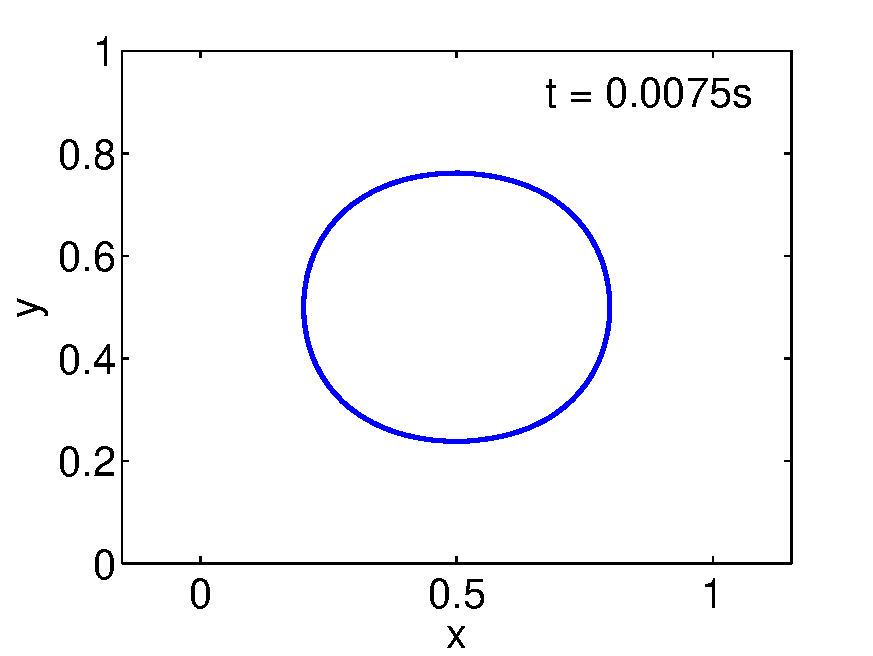
\includegraphics[width=.3\textwidth]{ellipse0075}\label{fig:ellipse3}}
	\subfigure[]{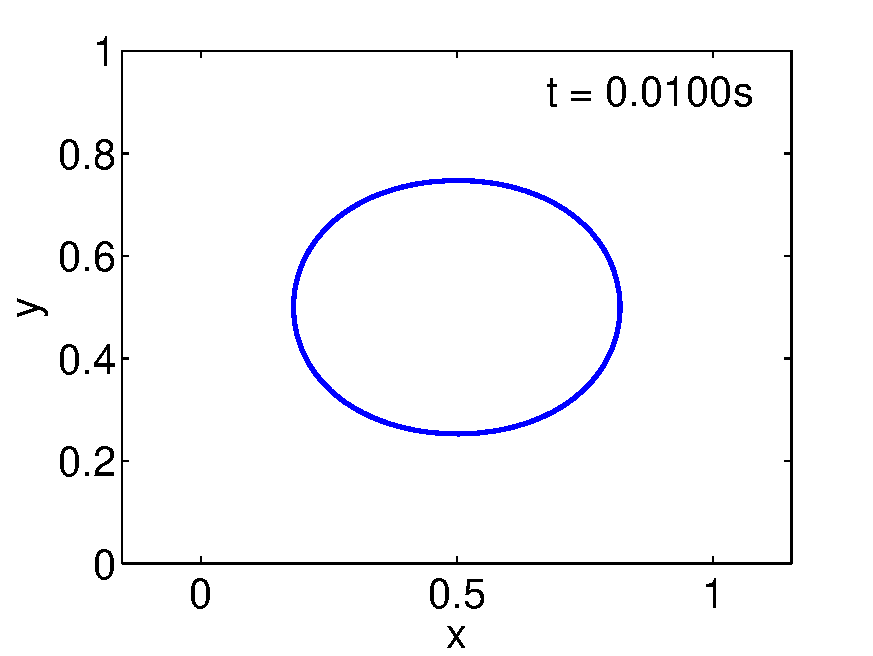
\includegraphics[width=.3\textwidth]{ellipse0100}\label{fig:ellipse4}}
	\subfigure[]{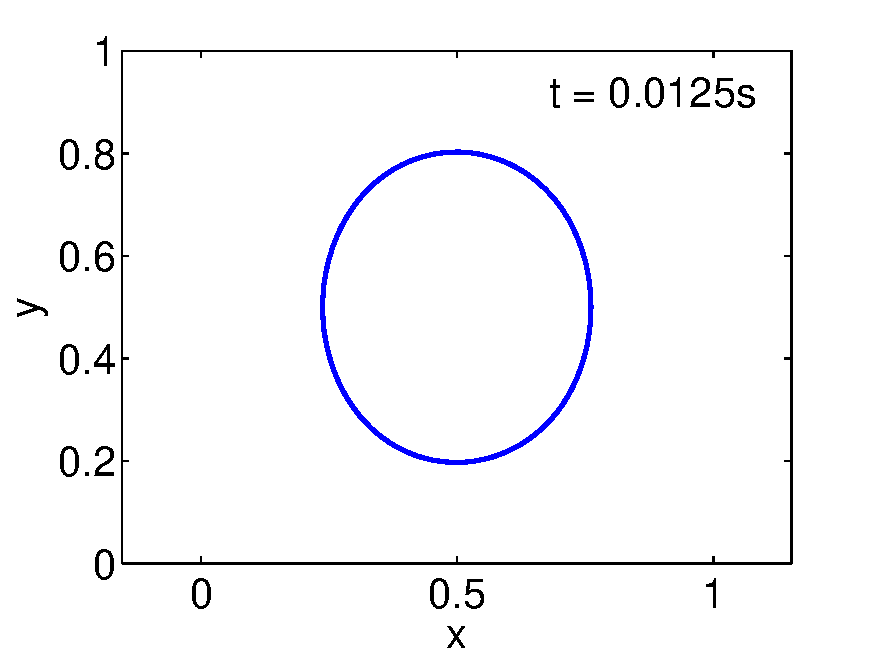
\includegraphics[width=.3\textwidth]{ellipse0125}\label{fig:ellipse5}}
  	\caption{Profiles of an elliptical membrane at different times. }
  	\label{fig:ellipseProfile}
\end{figure}

In this example, we are using Peskin's two-step numerical algorithm \cite{PeskinIB} which is implemented in the folder \emph{solver/Peskin-TwoStep/}. 
Since Matlab does not allow you to directly call functions residing in different folders, we need to add a couple folders to the PATH variable at the beginning of the script by executing
\footnote{{\bf Note:} This code is assuming that \emph{"cd ../../"} will bring you to \softwarename's root directory which is true when in the \emph{"examples/Elliptical Membrane} directory".}:
\begin{lstlisting}
% Add PATH reference in order to run solver
addpath('../../solver/Peskin-TwoStep');
addpath('../../solver/utils');
\end{lstlisting}
This will allow you to call the IB solver \emph{solver/Peskin-TwoStep/IBSolver.m} and other \emph{util} functions required by the solver. Since 
we are contaminating the PATH variable with directory references, we need to remove these references at the end of the script by executing:
\begin{lstlisting}
% Remove PATH reference to avoid clutter
rmpath('../../solver/Peskin-TwoStep');
rmpath('../../solver/utils');
\end{lstlisting}
If there are multiple solvers installed in \softwarename, removing the PATH references is essentially because of filename conflicts. For example, 
if there exist files named \emph{solver/Algorithm1/IBSolver.m} and \emph{solver/Algorithm2/IBSolver.m}, 
you will experience problems when both Algorithm1 and Algorithm2 are in your PATH variable. Therefore, you need to add and remove PATH references when 
changing algorithms.

Once your script correctly links to the IB solver, you need to call the function {\bf IBSolver}. This function takes several parameters as input:
\begin{itemize}
\item $\mu$ : Dynamic viscosity (scalar) in Navier-Stokes equation \eqref{eq:NSE}.
\item $\rho$ : Fluid density (scalar) in Navier-Stokes equation \eqref{eq:NSE}.
\item $\sigma$ : Spring constant (scalar) of the membrane defined in equation \eqref{eq:forceDensity}.
\item $L$ : Resting length (scalar) of the membrane defined in equation \eqref{eq:forceDensity}.

\item IC\_U, IC\_V: A function handle describing the initial velocity of the fluid $(u(\vec{x},0),v(\vec{x},0))$.
						The function needs to have the profile:\\
						\begin{center}{\bf U = IC\_U(X,Y);}\end{center}
						where X,Y are matrices defining points on the Eulerian grid (created by Matlab's {\bf meshgrid} function) and
						U is a matrix defining velocity in the x direction (or y direction).
\item IC\_ChiX,IC\_ChiY: A function handle describing the initial location of the membrane $(\chi_x(s,0),~\chi_y(s,0))$
							The function needs to have the profile:\\
							\begin{center}{\bf ChiX = IC\_ChiX(S);}\end{center}
							where S is a vector defining points on the Lagrangian grid $s\in[0,1]$ and
							ChiX is a vector defining points (in x direction or y direction) on the membrane.
							
\item $N$ : Number of grid points on each side of the square Eulerian grid.
\item $N_b$ : Number of grid points on membrane's Lagrangian grid.
\item NTime: Number of time steps in simulation.
\item Tfinal: The final time to compute the numerical solution to.

\item ActionFun: A function handle which is called after each time step. The functions
							needs to have the profile:\\
							\begin{center}{\bf ActionFun( dx, dt, indexT, X, Y, U, V, chiX, chiY, Fx, Fy);}\end{center}
							where 
							\begin{itemize}
								\item dx: The scalar spatial discretization of the Eulerian grid.
								\item dt: The scalar temporal discretization.
								\item indexT: The number of time steps that have been executed so far.
								\item X,Y: Matrices which define points on the Eulerian grid.
								\item U,V: Matrices containing the velocity of the fluid at the end of the current time step on the Eulerian grid. 
								\item chiX,chiY: Vectors defining points on the membrane using the Lagrangian grid $s\in[0,1]$ at the end of the 
										current time step.
							\end{itemize}
\end{itemize}
When the function {\bf IBSolver} finishes running, it will return $[X,~Y,~S,~U,~V,~chiX,~chiY]$ which are matrices of the Eulerian and Lagrangian grid,
the fluid velocity, and membrane position at the last time step.


\newpage

\bibliography{citations}
\bibliographystyle{plain}



\end{document}


